\documentclass[11pt,a4paper]{article}
\usepackage[a4paper,margin=25mm]{geometry}
\setcounter{tocdepth}{4}
\usepackage[utf8]{inputenc}
\usepackage[T1]{fontenc}
\usepackage{lmodern}
\usepackage{amsmath}
\usepackage{amsthm}
\usepackage{amssymb}
\usepackage{mathrsfs}
\usepackage{amsfonts}
\usepackage{stmaryrd}
\usepackage{xfrac}
\usepackage{dsfont}
\usepackage{fancybox}
\usepackage{fancyref}
\usepackage{multicol}
\usepackage{graphicx}
\usepackage{wrapfig}
\usepackage{textcomp}
\usepackage{mathrsfs}
\usepackage[svgnames]{xcolor}
\usepackage{color}
\usepackage{listings}
\usepackage{tikz-cd}
\usepackage[hidelinks]{hyperref}
\usepackage{cleveref}
\usepackage{comment}
\usepackage{caption}
\usepackage{shuffle}
\usepackage{multirow}
\usepackage{appendix}
\usepackage{fdsymbol}
\usepackage{float}
\usepackage{algorithm}
\usepackage[noend]{algpseudocode}

\newcommand{\HRule}{\rule{\linewidth}{0.5mm}}
\newcommand{\Dyck}[1]{\textsc{Dyck$_{#1}$}}
\newcommand{\FA}[1]{\textsc{FindAny$_{#1}$}}
\newcommand{\FFL}[1]{\textsc{FindFixedLength$_{#1}$}}
\newcommand{\FFP}[1]{\textsc{FindFixedPos$_{#1}$}}
\newcommand{\FALM}[1]{\textsc{FindAtLeftMost$_{#1}$}}
\newcommand{\FARM}[1]{\textsc{FindAtRightMost$_{#1}$}}
\newcommand{\FF}[1]{\textsc{FindFirst$_{#1}$}}
\newcommand{\Null}{\textsc{Null}}

\newcommand{\hered}[1]{\paragraph*{Induction:}{#1}}
\newcommand{\init}[1]{\paragraph*{Initialization:}{#1}}
\newcommand{\IH}[1]{\paragraph*{Induction Hypothesis:}{#1}}
\newcommand{\Conc}[1]{\paragraph*{Conclusion:}{#1}}
\newcommand{\remark}[1]{\paragraph*{Remark:}{#1}}
\newcommand{\observation}[1]{\paragraph*{Observation:}{#1}}
\newcommand{\notation}[1]{\paragraph*{Notation:}{#1}}
\newcommand{\property}[1]{\paragraph*{Property:}{#1}}

\renewcommand{\comment}[1]{}
\newcommand\blfootnote[1]{%
    \begingroup
    \renewcommand\thefootnote{}\footnote{#1}%
    \addtocounter{footnote}{-1}%
    \endgroup
}

\theoremstyle{definition}
\newtheorem{definition}{Définition}
\newtheorem{proposition}{Proposition}[definition]

\theoremstyle{plain}
\newtheorem{theorem}{Theorem}[section]
\newtheorem{corollary}{Corollary}[theorem]
\newtheorem{lemma}{Lemma}[theorem]

\theoremstyle{definition}
\newtheorem{conjecture}{Conjecture}[definition]
\newtheorem{cproof}{Proof Corollary}[theorem] 
\newtheorem{lproof}{Proof Lemma}[theorem]
\newtheorem{tproof}{Proof Theorem}[section]

\begin{document}

\begin{titlepage}
    \begin{sffamily}
        \begin{center}

            \textsc{\LARGE École Normale Supérieure de Lyon}\\[0.5cm]
            \textsc{\LARGE Latvijas Universit$\overline{\textrm{a}}$te} \\[1cm]

            \begin{minipage}[c]{.46\linewidth}
                \hspace{-2cm}
                
\includegraphics[width=9.5cm]{illustration/Logo_ENS_Lyon.png}
            \end{minipage}
            \hfill%
            \begin{minipage}[c]{.46\linewidth}
                \centering
                
\includegraphics[width=8cm]{illustration/Faculty_of_Computing_University_of_Latvia-1536x619-1.png}
            \end{minipage}\\[2cm]

            \textsc{\Large M1 Internship Repport}\\[2cm]

            \HRule \\[0.4cm]
            \textsc{\huge Complexity of recognizing Dyck language with a quantum computer.}
            \HRule \\[2cm]

            \vfill

            % Author and supervisor
            \hspace{-0.8cm}
            \begin{minipage}{0.4\textwidth}
                \begin{flushleft} \large
                    \emph{Student :} \\
                    Maxime \textsc{Cautrès}\\
                \end{flushleft}
            \end{minipage}
            \hspace{3cm}
            \begin{minipage}{0.4\textwidth}
                \begin{flushright} \large
                    \emph{Supervisor :} \\
                    Andris \textsc{Ambainis}\\
                    Kamil \textsc{Khadiev}\\
                \end{flushright}
            \end{minipage}

            \vspace*{0.5cm}

            % Bottom of the page
            {\large   May the 2nd 2022 -  July the 22th 2022}
        \end{center}
    \end{sffamily}
\end{titlepage}

\tableofcontents

\newpage




\section{Introduction}
\begin{itemize}
    \item presentation of the Internship
    \item state of the art
    \item result
    \item goal to reach
\end{itemize}


\section{Preliminaries}
\begin{itemize}
    \item Quantum Query Complexity
    \item \Dyck{k, n} problem
    \item Trichotomy statement
    \item Adversary methode
\end{itemize}



\section{A better algorithm for \Dyck{k,n}}

\subsection{A better Complexity Analysis of the original algorithm}

In the article \cite{art:2DGrid}, Andris Ambainis give us a quantum algorithm to recognize
the belonging of a $n$ length bit string in $\Dyck{k, n}$ using
$O(\sqrt{n}(\log_2(n))^{0.5k})$ quantum queries. But the quantum query complexity for $k=1$ is not as good as a
Grover's search which is sufficient. More precisely, for $k=1$ the algorithm is
searching for a minimal $\pm 2$ string in $1x0$ but we know that every minimal $\pm 2$ string
is of size $2$. So the logarithmic search of the upper bound on the size of the
minimal $\pm 2$ string is no more useful and the algorithm can be summarized to
applying a Grover search for 2 consecutive 0 or two consecutive 1. This lower the quantum
query complexity of the initial case of the function to $O(\sqrt{n})$ instead of $O(\sqrt{n\log_2(n)})$.
This give us this following algorithm for \FA{k}.

\begin{algorithm}
    \caption{\FA{k}(l,r,s)}\label{alg:FA_prim}
    \begin{algorithmic}
        \Require $0 \leq l < r$ and $s \subseteq \{1,-1\}$
        \If{$k > 2$}
        \State \textbf{Find} $d$ in $\{2^{\lceil \log_2(k)\rceil }, 2^{\lceil \log_2(k)+1\rceil },\ldots,2^{\lceil \log_2(r-l)\rceil }\}$
        such that \\
        \hspace*{1cm} $v_d \gets $ \FFL{k}$(l,r,d,s)$ is \textbf{not} \Null
        \State \textbf{return} $v_d$ or \Null \ if none
        \Else
        \State \textbf{Find} $t$ in $\{l, l+1, \dots, r\}$ such that \\
        \hspace*{1cm} $v_t \gets$ \FALM{2}$(l,r,t,2,s)$ is \textbf{not} \Null
        \State \textbf{return} $v_t$ of \Null if none
        \EndIf
    \end{algorithmic}
\end{algorithm}

The same improvement can be done on \FFP{k} because if $k = 2$ the logarithmic
search is useless. So \FFP{k} can be redefined as in \textsc{Algorithm} \autoref{alg:ffp_better}.
For $k=2$, the complexity is lowered from $O(\sqrt{\log_2(l-r)})$ to $O(1)$.

\begin{algorithm}
    \caption{$\FFP{k}(l,r,t,s)$}\label{alg:ffp_better}
    \begin{algorithmic}
        \Require $0\leq l<r$, $l \leq t \leq r$ and $s \subseteq \{1, -1\}$
        \If{$k>2$}
        \State \textbf{Find} $d$ in $\{2^{\lceil \log_2(k)\rceil }, 2^{\lceil \log_2(k)+1\rceil },\ldots,2^{\lceil \log_2(r-l)\rceil }\}$
        such that \\
        \hspace*{1cm} $v_d \gets $ \FALM{k}$(l,r,t,d,s)$ is \textbf{not} \Null
        \State \textbf{return} $v_d$ or \Null \ if none
        \Else
        \ $v \gets $ \FALM{k}$(l,r,t,2,s)$ is \textbf{not} \Null
        \State \textbf{return} $v_d$ or \Null \ if none
        \EndIf
    \end{algorithmic}
\end{algorithm}

This small improvements on the initial cases will improve the global
quantum query complexity of each subroutine and finally the quantum
query complexity for \Dyck{k,n}.

\newpage

\begin{theorem}{\textbf{\Dyck{k,n}'s algorithm correctness}} \label{th:subroutine_correctness}
    The new definition of \FA{} and \FFP{} does not change the behavior the original algorithm.
\end{theorem}

\begin{tproof}
    The behavior of the \Dyck{k,n} algorithm with the new subroutines is the same than the older
    one as \FA{} (resp. \FF{}) has the same sub-behavior on every entry with its
    older definition.
\end{tproof}

\begin{theorem}{\textbf{\Dyck{k,n}'s Subroutines complexity}} \label{th:subroutine_complexity}
    The subroutines' quantum query complexity for $k$ are the following.
    \begin{enumerate}
        \item $Q$(\Dyck{k,n}) = $O\left(\sqrt{n}(\log_2(n))^{0.5(k-1)}\right)$ \ for $k \geq 1$
        \item $Q$(\FA{k+1}$(l,r,s)$) = $O\left(\sqrt{r-l}(\log_2(r-l))^{0.5(k-1)}\right)$ \ for $k \geq 1$
        \item $Q$(\FFL{k+1}$(l,r,d,s)$) = $O\left(\sqrt{r-l}(\log_2(r-l))^{0.5(k-2)}\right)$ \ for $k \geq 2$
        \item $Q$(\FALM{k+1}$(l, r, t, d, s)$) = $\left\{
                  \begin{array}{l}
                      O\left(\sqrt{d}(\log_2(d))^{0.5(k-2)}\right)\ \textrm{for} \ k \geq 2 \\
                      O(1)\ \textrm{for} \  k = 1
                  \end{array}
                  \right.$
        \item $Q$(\FF{k}$(l,r,s, left)$) = $O\left(\sqrt{r-l}(\log_2(r-l))^{0.5(k-2)}\right)$ \ for $k \geq 2$
        \item $Q$(\FFP{k}$(l,r,t,s)$) = $\left\{ \begin{array}{l}
                      O\left(\sqrt{r-l}(\log_2(r-l))^{0.5(k-2)}\right)\ \textrm{for} \ k \geq 3 \\
                      O(1) \ \textrm{for} \ k = 2
                  \end{array}
                  \right.$
    \end{enumerate}
\end{theorem}

Unfortunately, the improvements done on the initial cases of some of the subroutines are not sufficient
to get a significant improvement for the quantum query complexity of \Dyck{k,n} algorithm. In order to
improve more the query complexity, an other algorithm using a different strategy should be found.

\subsection{A new algorithm for \Dyck{2,n}}

First, we would like to find an algorithm with a quantum query complexity near to match the lower bound,
$\exists c \geq 1$ such that $Q\left(\Dyck{k,n}\right)=\Omega\left(\sqrt{n}c^k\right)$, describes by Andris
Ambainis team in \cite{art:2DGrid}. This means that we are searching for an algorithm with a quantum query
complexity of $O\left(\sqrt{n}\right)$.

If we come back to the case were $k=1$, the query complexity comes only from a call to Grover's search
because rejecting is easily by finding a 00 or a 11 substrings inside the entry. For $k=2$
it no more possible as the substrings that reject are of the form 00(10)*0 or of the form 11(01)*1. It
implies that the number of calls to Grover's search in the naive approach is in $O\left(n\right)$ so the
quantum query complexity finally becomes $O\left(n\sqrt{n}\right)$. In order to keep it in
$O\left(\sqrt{n}\right)$, the algorithm must do a constant number of calls to Grover's search.

For that, we will  define a new alphabet that allow to express every even length binary
strings and that will have convenient property compatible with Grover's search. Let
$\mathcal{A} = \{a, b, c, d\}$ the alphabet where $a$ corresponds to 00, $b$ to 11, $c$
to 01, and $d$ to 10. So every string of size 2 has its letter in $\mathcal{A}$ thus every
even length bit string is expressed in $\mathcal{A}^*$.

This alphabet $\mathcal{A}$ is important because each of this letter has a height variation
in $\{-2, 0, 2\}$. Indeed, $a$ has a 2 height variation, $b$ a $-2$, $c$ a 0, and $d$ a zero.
This means that after each letter in a word, the current height will be even. Moreover,
for a valid Dyck word of height at most 2, after every letter the height will be 0 or 2
which are respectively the lower and upper bound for the height. It means that no letter
can cross a border between its two bits.

\begin{figure}[htb]
    \centering
    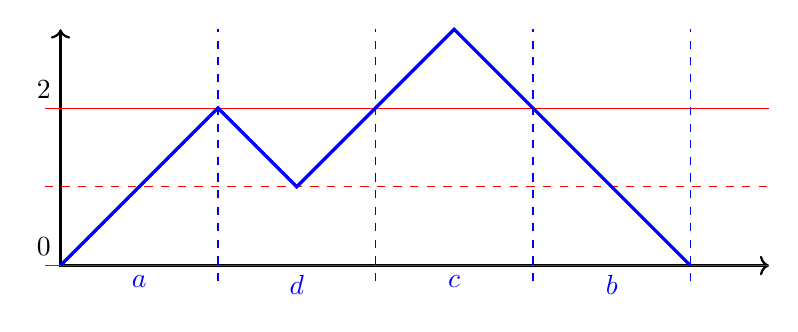
\begin{tikzpicture}
        \draw[<->, thick] (0, 3) -- (0, 0) -- (9, 0);
        \draw[dashed, red] (-.2, 1) --(9, 1);
        \draw[red] (-.2, 2) --(9, 2);
        \draw[red] (-.2, 0) --(9, 0);
        \draw[very thick, blue] (0, 0) -- (2, 2) -- (3, 1) -- (5, 3) -- (8, 0);
        \draw[blue, dashed] (2, -.2) -- (2, 3);
        \draw[blue, dashed] (4, -.2) -- (4, 3);
        \draw[blue, dashed] (6, -.2) -- (6, 3);
        \draw[blue, dashed] (8, -.2) -- (8, 3);
        \draw[blue] (1, 0) node[below] {$a$};
        \draw[blue] (3, 0) node[below] {$d$};
        \draw[blue] (5, 0) node[below] {$c$};
        \draw[blue] (7, 0) node[below] {$b$};
        \draw (0, 2) node[above left] {2};
        \draw (0, 0) node[above left] {0};
    \end{tikzpicture}
    \caption{Illustration of the letters of $\mathcal{A}$ using Dyck's representation.}
    \label{tikz:dyck2alphabet}
\end{figure}

This property is important as it implies that every $\pm 3$ strings uses at least two letter.


\newpage

\section{Conclusion}

bonsoir paris

bonnoaisn

boabdado

ibabdiubaoiz

iabdiabdo


\bibliographystyle{plain}
\bibliography{biblio}

\newpage

\section{Appendix}

\begin{appendix}

    \section*{The frame of the intership}

    \section{The algorithm for \Dyck{k, n}}

    \begin{algorithm}
        \caption{\Dyck{k,n}}\label{alg:dyck_kn}
        \begin{algorithmic}
            \Require $n \geq 0$ and $k \geq 1$
            \Ensure $|x| = n $
            \State $x \gets 1^kx0^k$
            \State $v \gets$ \FA{k+1}$(0, n+2*k-1, \{1,-1\})$
            \State \textbf{return} v = \Null
        \end{algorithmic}
    \end{algorithm}

    \begin{algorithm}
        \caption{\FA{k}$(l,r,s)$}\label{alg:fa_k}
        \begin{algorithmic}
            \Require $0 \leq l < r$ and $s \subseteq \{1,-1\}$
            \State \textbf{Find} $d$ in $\{2^{\lceil \log_2(k)\rceil }, 2^{\lceil \log_2(k)+1\rceil },\ldots,2^{\lceil \log_2(r-l)\rceil }\}$
            such that \\
            \hspace*{1cm} $v_d \gets $ \FFL{k}$(l,r,d,s)$ is \textbf{not} \Null
            \State \textbf{return} $v_d$ or \Null \ if none
        \end{algorithmic}
    \end{algorithm}

    \begin{algorithm}
        \caption{\FFL{k}$(l,r,d,s)$}\label{alg:ffl_k}
        \begin{algorithmic}
            \Require $0 \leq l < r$, $1\leq d \leq r-l$ and $s \subseteq \{1,-1\}$
            \State \textbf{Find} $t$ in $\{l, l+1, \dots, r\}$ such that \\
            \hspace*{1cm} $v_t \gets$ \FALM{k}$(l,r,t,d,s)$ is \textbf{not} \Null
            \State \textbf{return} $v_t$ of \Null if none
        \end{algorithmic}
    \end{algorithm}

    \begin{algorithm}
        \caption{\FALM{k}$(l,r,d,t,s)$}\label{alg:falm_k}
        \begin{algorithmic}
            \Require $0 \leq l < r$, $l \leq r \leq r$, $1\leq d \leq r-l$ and $s \subseteq \{1,-1\}$
            \State $v = (i_1,j_1,\sigma_1) \gets \FALM{k-1}(l,r,t,d-1,\{1,-1\})$
            \If{$v \neq \Null$} {
                \State $v' = (i_2,j_2,\sigma_2) \gets \FARM{k-1}(l,r,i_1-1,d-1,\{1,-1\})$
                \If{$v' = \Null$}
                \State $v' = (i_2,j_2,\sigma_2) \gets \FF{k-1}(\max(l, j_1-d+1),i_1-1,\{1,-1\}, left)$
                \EndIf
                \If{$v'\neq \Null$ and $\sigma_2 \neq \sigma_1$}{\ $v' \gets \Null$}
                \EndIf
                \If{$v' = \Null$}
                \State $v' = (i_2,j_2,\sigma_2) \gets \FALM{k-1}(l,r,j_1+1,d-1,\{1,-1\})$
                \EndIf
                \If{$v' = \Null$}
                \State $v' = (i_2,j_2,\sigma_2) \gets \FF{k-1}(j_1+1,\max(r, i_1+d-1),\{1,-1\}, right)$
                \EndIf
                \If{$v' = \Null$}{\ \textbf{return} \Null}
                \EndIf
            }
            \Else {
            \State $v = (i_1,j_1,\sigma_1) \gets \FF{k-1}(t, min(t+d-1, r), \{1,-1\}, right)$
            \If{v = \Null}{\ \textbf{return} \Null}
            \EndIf
            \State $v' = (i_2, j_2, \sigma_2) \gets \FF{k-1}(max(t-d+1, l), t, \{1, -1\}, left)$
                \If{$v' = \Null$}{\ \textbf{return} \Null}
                \EndIf
                }
                \EndIf
                \If{$\sigma_1=\sigma_2$ and $\sigma_1 \in s$ and $\max(j_1, j_2) - \min(i_1, i_2) + 1 \leq d$}
                \State \textbf{return} $(\min(i_1, i_2), \max(j_1, j_2), \sigma_1)$
            \Else{\ \textbf{return} \Null}
            \EndIf

        \end{algorithmic}
    \end{algorithm}

    \begin{algorithm}
        \caption{\FF{k}$(l, r, s, left)$}
        \begin{algorithmic}
            \Require $0\leq l < r$ and $s \subseteq \{1,-1\}$
            \State $lBorder \gets l, rBorder \gets r, d \gets 1$
            \While{$lBorder + 1 < rBorder $}
            \State $ mid \gets \lfloor (lBorder + rBorder)/2 \rfloor $
            \State $v_l \gets \FA{k}(lBorder, mid, s)$
            \If{$v_l \neq \Null$}{\ $rBorder \gets mid$}
            \Else
            \State $v_{mid} \gets \FFP{k}(lBorder, rBorder, mid, s, left)$
            \If{$v_{mid} \neq \Null$}{\ \textbf{return} $v_{mid}$}
            \Else{\ $lBorder \gets mid + 1$}
            \EndIf
            \EndIf
            \State $d \gets d+1$
            \EndWhile
            \State \textbf{return} \Null
        \end{algorithmic}
    \end{algorithm}


    \begin{algorithm}
        \caption{$\FFP{k}(l,r,t,s)$}
        \begin{algorithmic}
            \Require $0\leq l<r$, $l \leq t \leq r$ and $s \subseteq \{1, -1\}$

            \State \textbf{Find} $d$ in $\{2^{\lceil \log_2(k)\rceil }, 2^{\lceil \log_2(k)+1\rceil },\ldots,2^{\lceil \log_2(r-l)\rceil }\}$
            such that \\
            \hspace*{1cm} $v_d \gets $ \FALM{k}$(l,r,t,d,s)$ is \textbf{not} \Null
            \State \textbf{return} $v_d$ or \Null \ if none
        \end{algorithmic}
    \end{algorithm}

    \section{The proof of the quantum query complexity for \Dyck{k,n} algorithm's subroutines}

    \begin{tproof} The proof is done by induction on the height of the Dyck word $k$.
        \init{For $k=1$ and $k=2$ we have the following initialization. \\
            \begin{itemize}
                \item For $k=1$, only \FALM{2}, \FA{2} ,and \Dyck{1,n} are defined. The $O(1)$ quantum query complexity
                      of \FALM{2} comes directly from the definition of its initial case, as the $O(\sqrt{r-l})$ quantum
                      query complexity of \FA{2}. Then the $O\left(\sqrt{n}\right)$ quantum query complexity of \Dyck{1,n} comes from
                      the call to \FA{2}.
                \item For $k=2$, the inductive part of the algorithm start and every subroutines is defined. The $O(1)$
                      quantum query complexity of \FFP{2} comes from the call to \FALM{2}.
                      The $O\left(\sqrt{r-l}\right)$ quantum query complexity of \FF{2} comes from the dichotomize search using \FA{2} and
                      \FFP{2} because $\sum_{u=1}^{log_2(r-l)}2u\left(O\left(\sqrt{\frac{r-l}{2^{u-1}}}\right)+O(1)\right) = O(\sqrt{r-l})$
                      (Detailed in the induction). The $O(\sqrt{d})$ quantum query complexity of \FALM{3} comes from the
                      constant amount of calls to \FF{2} and \FALM{2} with entry of size $d$. The $O(\sqrt{r-l})$ quantum query
                      complexity of \FFL{3} comes from the $O\left(\sqrt{\frac{r-l}{d}}\right)$ calls to \FALM{3}. The $O\left(\sqrt{(r-l)\log_2(r-l)}\right)$
                      quantum query complexity of \FA{3} comes from the $O\left(\sqrt{\log_2(r-l)}\right)$ calls to \FFL{3}. Finally, the
                      $O\left(\sqrt{(r-l)\log_2(r-l)}\right)$ quantum query complexity of \Dyck{2} comes from the call to \FA{3}.
            \end{itemize}
        }
        \hered{Let suppose it exists $k$ such that \autoref{th:subroutine_complexity} is
            true for $k$. Let prove that it is true for $k+1$. \\

            First, the $O\left(\sqrt{r-l}(\log_2(r-l))^{0.5(k-1)}\right)$ quantum query complexity of \FFP{k+1} comes from
            the $O\left(\sqrt{\log(r-l)}\right)$ calls to \FALM{k+1}.
            \begin{align*}
                Q(\textrm{\FFP{k+1}}(l, r, t, s)) & = O(\sqrt{\log(r-l)}) \times O\left(Q(\textrm{\FALM{k+1}}(l, r, t, d, s))\right)\            \\
                                                  & \overset{IH}{=} O \left( \sqrt{\log(r-l)} \times \sqrt{r-l}(\log_2(r-l))^{0.5(k-2)}  \right) \\
                                                  & = O \left( \sqrt{r-l}(\log_2(r-l))^{0.5(k-1)} \right)
            \end{align*}

            Thus the $O \left(\sqrt{r-l}(\log_2(r-l))^{0.5(k-2)}\right)$ quantum query complexity of \FF{k+1} comes
            from the dichotomize search using calls to \FA{k+1} and \FF{k+1}.

            \begin{align*}
                Q(\textrm{\FF{k+1}}(l,r,t,d,s)) & = \begin{array}{l}
                    \sum_{u=1}^{\log_2(r-l)}2u \times O\left(Q(\textrm{\FA{k+1}}(0, \frac{r-l}{2^{u-1}}, s))\right) \\
                    + \sum_{u=1}^{\log_2(r-l)}2u \times O\left(Q(\textrm{\FFP{k+1}}(0, \frac{r-l}{2^{u-1}}, \_ , s, left))\right)
                \end{array}                                                     \\
                                                & \overset{IH}{=}
                O\left(\sum_{u=1}^{\log_2(r-l)}2u \times \sqrt{\frac{r-l}{2^{u-1}}}(\log_2(\frac{r-l}{2^{u-1}}))^{0.5(k-1)}\right) \\
                                                & =
                O\left(\sum_{u=1}^{\log_2(r-l)}2u \times \sqrt{\frac{r-l}{2^{u-1}}}(\log_2(r-l))^{0.5(k-1)}\right)                 \\
                                                & =
                O \left(\sqrt{r-l}(\log_2(r-l))^{0.5(k-1)}\sum_{u=1}^{\log_2(r-l)}u\times (\frac{1}{\sqrt{2}})^{u-1} \right)       \\
                                                & =^{a}
                O \left(\sqrt{r-l}(\log_2(r-l))^{0.5(k-1)} \frac{\sqrt{2}^2}{(\sqrt{2}-1)^2}\right)                                \\
                                                & =
                O \left(\sqrt{r-l}(\log_2(r-l))^{0.5(k-1)}\right)
            \end{align*}

            \blfootnote{\begin{align*}
                    ^{a}\sum_{u=1}^{+\infty} \left(\frac{\textrm{d}}{\textrm{d}x}(x^{u})\right)\left(\frac{1}{\sqrt{2}}\right)
                    \leq \left(\frac{\textrm{d}}{\textrm{d}x} \left( \sum_{u=1}^{+\infty} x^u \right)\right)\left(\frac{1}{\sqrt{2}}\right)
                    \leq \left(\frac{\textrm{d}}{\textrm{d}x} \left( \frac{x}{1-x} \right)\right)\left(\frac{1}{\sqrt{2}}\right)
                    \leq \left(\frac{1}{(1-x)^2}\right)\left(\frac{1}{\sqrt{2}}\right)
                    \leq \frac{1}{(1-\frac{1}{\sqrt{2}})^2} \leq \frac{\sqrt{2}^2}{(\sqrt{2} - 1)^2}
                \end{align*}}

            Next, the $ O\left(\sqrt{d}(\log_2(d))^{0.5(k-1)} \right)$ quantum query complexity comes of \FALM{k+2}from the constant amount
            of calls to \FALM{k+1}, \FARM{k+1} ,and \FF{k+1}.

            \begin{align*}
                Q(\textrm{\FALM{k+2}}(l,r,t,d,s)) & = \begin{array}{l}
                    3 \times O\left(Q(\textrm{\FALM{k+1}}(l,r,t,d,\{1,-1\}))\right) \\
                    + 4 \times O\left(Q(\textrm{\FF{k+1}}(l,r,\{1,-1\},left))\right)
                \end{array}                                  \\
                                                  & \overset{IH}{=} O\left(\sqrt{d}(\log_2(d))^{0.5(k-1)} \right)
            \end{align*}

            After that, the $O\left( \sqrt{r-l}(\log_2(r-l))^{0.5(k-1)}\right)$ quantum query complexity of \FFL{k+2} comes from the
            $O\left(\sqrt{\frac{r-l}{d}}\right)$ calls to \FALM{k+2}.

            \begin{align*}
                Q(\textrm{\FFL{k+2}}(l, r, d, s)) & = O\left(\sqrt{\frac{r-l}{d}}\right) \times O\left(Q(\textrm{\FALM{k+2}}(l,r,t,d,s))\right) \\
                                                  & = O\left( \sqrt{\frac{r-l}{d}} \times \sqrt{d}(\log_2(d))^{0.5(k-1)}\right)                 \\
                                                  & = O\left( \sqrt{r-l}(\log_2(d))^{0.5(k-1)}\right)                                           \\
                                                  & = O\left( \sqrt{r-l}(\log_2(r-l))^{0.5(k-1)}\right)
            \end{align*}

            Hence the $O\left( \sqrt{r-l}(\log_2(r-l))^{0.5k} \right)$ quantum query complexity of \FA{k+2} comes from the
            the $O\left(\sqrt{\log_2(r-l)}\right)$ calls to \FFL{k+2}

            \begin{align*}
                Q(\textrm{\FA{k+2}}(l, r, s)) & = O\left(\sqrt{\log(r-l)}\right) \times O\left(Q(\textrm{\FFL{k+2}}(l, r, d, s))\right) \\
                                              & = O\left( \sqrt{\log(r-l)} \times \sqrt{r-l}(\log_2(r-l))^{0.5(k-1)} \right)            \\
                                              & = O\left( \sqrt{r-l}(\log_2(r-l))^{0.5k} \right)                                        \\
            \end{align*}

            Finally, the $O\left( \sqrt{n}(\log_2(n))^{0.5k} \right)$ quantum query complexity of \Dyck{k+1,n} comes from the
            call to \FA{k+2}.

            \begin{align*}
                Q(\textrm{\Dyck{k+1,n}}) & = O\left(Q(\textrm{\FA{k+2}}(0,n+2k+1,s))\right) \\
                                         & = O\left(Q(\textrm{\FA{k+2}}(0, n, s))\right)    \\
                                         & = O\left( \sqrt{n}(\log_2(n))^{0.5k} \right)
            \end{align*}

        }

        \Conc{By the induction principle we get that the \autoref{th:subroutine_complexity} is true for $k \in \mathbb{N}^*$}
    \end{tproof}

\end{appendix}

\end{document}